\documentclass{article}
\usepackage{graphicx} % Required for inserting images
\usepackage{listings}
\usepackage{xcolor}
\usepackage{subfigure} 
\usepackage{amsmath}
\usepackage{booktabs}
\usepackage[left=3cm,right=3cm,top=3cm,bottom=3cm]{geometry}

% Define colors for syntax highlighting
\definecolor{keyword}{RGB}{0,0,255}
\definecolor{comment}{RGB}{0,128,0}
\definecolor{string}{RGB}{163,21,21}
\definecolor{background}{RGB}{240,240,240}

\lstset{
    language=Python,
    basicstyle=\ttfamily\small,
    keywordstyle=\color{keyword}\bfseries,
    commentstyle=\color{comment},
    stringstyle=\color{string},
    backgroundcolor=\color{background},
    frame=single,
    breaklines=true,
    numbers=left,
    numberstyle=\tiny\color{gray},
    captionpos=b,
    tabsize=4,
    showspaces=false,
    showstringspaces=false,
    escapeinside={(*@}{@*)}
}

\begin{document}

% Title and Information
\vspace{-8 cm}
\centering
\large \textbf{\fontsize{18}{22}\selectfont EC6103E Applied Mathematics\\ for Electronics Design}\\
\vspace{0.5 cm}
\large \textbf{\fontsize{18}{18}\selectfont Project-1 Report}\\
\vspace{0.6cm}
\large \textbf{\fontsize{22}{27}\selectfont Image Denoising Using\\ Patch-Based SVD}\\
\vspace{0.4cm}

\begin{tabular}{p{6.2cm} l}
\textbf{\fontsize{14}{16}\selectfont R. Jivith Abhishek} & \textbf{\fontsize{16}{16}\selectfont M260957EC} \\[0.3cm]
\textbf{\fontsize{14}{16}\selectfont Raghuveer Singh} & \textbf{\fontsize{16}{16}\selectfont M260960EC} \\[0.3cm]
\textbf{\fontsize{14}{16}\selectfont Palla Dali Naidu} & \textbf{\fontsize{16}{16}\selectfont M260465EC} \\
\end{tabular}\\
\vspace{0.4cm}
\large \textbf{\fontsize{14}{12}\selectfont Course faculty: Dr. SUDHISH N. GEORGE}\\

% Image insertion
\vspace{0.4cm}
\begin{figure}[ht!]
    \centering
    
\includegraphics[width= 0.4 \linewidth]{nit.jpg} 
\end{figure}

% Department Information
\vspace{0.6cm}
\textbf{\fontsize{14}{12}\selectfont DEPARTMENT OF ELECTRONICS AND COMMUNICATION ENGINEERING}\\
\vspace{0.3 cm}
\large \textbf{\fontsize{14}{12}\selectfont NATIONAL INSTITUTE OF TECHNOLOGY, CALICUT-673601}\\
\vspace{0.3 cm}
\textbf{\fontsize{14}{12}\selectfont MONSOON 2026}

\newpage

\begin{flushleft}

\section{Aim}
The aim of this project is to remove additive Gaussian noise from a grayscale image using patch-based Singular Value Decomposition (SVD). Three denoising strategies are implemented and compared: (i) rank-3 truncation, (ii) adaptive soft thresholding of singular values, and (iii) a hybrid 1-6-1 method that keeps the first singular value, soft-thresholds the next six and discards the last. The methods are evaluated using Mean Squared Error (MSE), Peak Signal-to-Noise Ratio (PSNR) and the fraction of singular-value energy retained.
\\

\section{Algorithm Description}
\subsection*{a. Setup and Image Acquisition:}
\begin{itemize}
    \item Import the required libraries: NumPy for numerical computation and SVD, Matplotlib for plotting and Pillow for reading the image.
    \item Load the test image (\texttt{cameraman.jpg}) and convert it to grayscale.
    \item Normalise pixel intensities to the range $[0, 1]$. The image size is $512 \times 512$.
\end{itemize}

\subsection*{b. Noise Generation:}
\begin{itemize}
    \item Generate zero-mean white Gaussian noise with standard deviation $\sigma = 0.05$ using a fixed random seed (42) for reproducibility.
    \item Add the noise to the original image and clip the result to $[0, 1]$ to obtain the noisy image.
\end{itemize}

\subsection*{c. Patch Extraction:}
\begin{itemize}
    \item Divide the noisy image into overlapping patches of size $8 \times 8$ with a stride of 4 pixels, giving $127 \times 127 = 16129$ patches.
    \item Process every patch independently using its SVD, $P = U \Sigma V^{T}$.
\end{itemize}

\subsection*{d. Singular Value Modification:}
For each patch the singular values $s_1 \geq s_2 \geq \dots \geq s_8$ are modified by one of the following methods:
\begin{itemize}
    \item \textbf{Rank-3 truncation:} keep $s_1, s_2, s_3$ unchanged and set $s_4, \dots, s_8$ to zero.
    \item \textbf{Adaptive soft thresholding:} every singular value is shrunk as $\tilde{s}_i = \max(s_i - \tau,\, 0)$, where the patch threshold depends on the patch activity:
    \begin{align*}
        \tau_0 &= \alpha \, \sigma \left(\sqrt{n} + \sqrt{n}\right), \quad n = 8, \\
        \text{activity} &= \frac{\max(\mathrm{var}(P) - \sigma^2,\, 0)}{\mathrm{var}(P) + \epsilon}, \\
        \tau &= \tau_0 \left(1 - \gamma \cdot \text{activity}\right),
    \end{align*}
    with $\alpha = 0.50$, $\gamma = 0.45$ and $\epsilon = 10^{-12}$. Smooth patches therefore receive a stronger threshold, and textured (high-activity) patches a weaker one.
    \item \textbf{Hybrid 1-6-1:} keep $s_1$ unchanged, soft-threshold $s_2, \dots, s_7$ with the same adaptive threshold $\tau$, and set $s_8$ to zero.
\end{itemize}

\subsection*{e. Reconstruction:}
\begin{itemize}
    \item Rebuild each denoised patch as $\hat{P} = U \tilde{\Sigma} V^{T}$.
    \item Add the patch estimates back at their original positions and divide by the number of patches covering each pixel (averaging of overlapping estimates).
    \item Clip the final image to $[0, 1]$.
\end{itemize}

\subsection*{f. Evaluation:}
\begin{itemize}
    \item Compute the MSE between the original image and each result:
    $\mathrm{MSE} = \frac{1}{MN}\sum (I - \hat{I})^2$.
    \item Compute the PSNR (peak value 1): $\mathrm{PSNR} = 10 \log_{10}\left(1 / \mathrm{MSE}\right)$ dB.
    \item Compute the average fraction of singular-value energy retained, $\sum \tilde{s}_i^2 / \sum s_i^2$, over all patches.
    \item Plot the average singular values before and after processing, together with the MSE, PSNR and energy-retention comparisons.
\end{itemize}
\newpage

\section{Code}
\begin{lstlisting}[caption={Importing libraries}]
import numpy as np
import matplotlib.pyplot as plt
from PIL import Image
\end{lstlisting}

\begin{lstlisting}[caption={Image and algorithm parameters}]
# Image and algorithm parameters


IMAGE_PATH = r"cameraman.jpg"

PATCH_SIZE = 8
STRIDE = 4

SIGMA = 0.05
RANDOM_SEED = 42

ALPHA = 0.50
GAMMA = 0.45

EPSILON = 1e-12
\end{lstlisting}

\begin{lstlisting}[caption={Loading the image and converting it to normalised grayscale}]
# Load the image

image = Image.open(IMAGE_PATH)
image = image.convert("L")

original = np.asarray(image, dtype=np.float64)
original = original / 255.0

print("Image dimensions:", original.shape)
print("Minimum pixel value:", original.min())
print("Maximum pixel value:", original.max())
\end{lstlisting}

\begin{lstlisting}[caption={Generating Gaussian noise and creating the noisy image}]
# Generate Gaussian noise

rng = np.random.default_rng(RANDOM_SEED)

noise = rng.normal(
    loc=0.0,
    scale=SIGMA,
    size=original.shape
)

noisy = original + noise
noisy = np.clip(noisy, 0.0, 1.0)
\end{lstlisting}

\begin{lstlisting}[caption={Patch-based SVD denoising function (rank-3, adaptive and hybrid 1-6-1)}]
# Patch-based SVD denoising

def svd_denoise(
    noisy_image,
    method,
    patch_size=8,
    stride=4,
    sigma=0.05,
    alpha=0.50,
    gamma=0.45
):

    height, width = noisy_image.shape

    # Store reconstructed patch estimates
    result_sum = np.zeros_like(noisy_image)

    # Count how many patches contribute to each pixel
    count = np.zeros_like(noisy_image)

    # Store singular values for analysis
    singular_value_sum = np.zeros(patch_size)
    modified_value_sum = np.zeros(patch_size)

    # Store energy retention for each patch
    energy_retention = []

    # Base threshold for adaptive soft thresholding
    tau0 = alpha * sigma * (
        np.sqrt(patch_size) + np.sqrt(patch_size)
    )

    # Process overlapping patches
    for row in range(0, height - patch_size + 1, stride):

        for col in range(0, width - patch_size + 1, stride):

            patch = noisy_image[
                row:row + patch_size,
                col:col + patch_size
            ]

            # Calculate SVD
            U, s, VT = np.linalg.svd(
                patch,
                full_matrices=False
            )

            # Rank-3 truncation
            if method == "rank3":

                s_new = np.zeros_like(s)
                s_new[:3] = s[:3]

            # Calculate adaptive threshold for the patch
            elif method in ("adaptive", "hybrid"):

                variance = np.var(patch)

                numerator = max(
                    variance - sigma**2,
                    0.0
                )

                denominator = variance + EPSILON

                activity = numerator / denominator

                threshold = tau0 * (
                    1.0 - gamma * activity
                )

                # Adaptive soft thresholding
                if method == "adaptive":

                    s_new = np.maximum(
                        s - threshold,
                        0.0
                    )

                # Hybrid 1-6-1 method
                elif method == "hybrid":

                    s_new = np.zeros_like(s)

                    # Keep the first singular value unchanged
                    s_new[0] = s[0]

                    # Soft-threshold the middle six singular values
                    s_new[1:7] = np.maximum(
                        s[1:7] - threshold,
                        0.0
                    )

                    # The final singular value remains zero

            else:
                raise ValueError(
                    "Method must be 'rank3', 'adaptive', or 'hybrid'"
                )

            # Collect singular values
            singular_value_sum += s
            modified_value_sum += s_new

            # Calculate the fraction of singular-value energy retained
            original_energy = np.sum(s**2)
            retained_energy = np.sum(s_new**2)

            if original_energy > EPSILON:

                energy_retention.append(
                    retained_energy / original_energy
                )

            # Reconstruct the denoised patch
            patch_result = (U * s_new) @ VT

            # Accumulate overlapping patch estimates
            result_sum[
                row:row + patch_size,
                col:col + patch_size
            ] += patch_result

            # Count how many patches contribute to each pixel
            count[
                row:row + patch_size,
                col:col + patch_size
            ] += 1

    # Average overlapping estimates
    denoised = result_sum / np.maximum(count, 1)

    # Keep original noisy pixels where no patch was processed
    denoised[count == 0] = noisy_image[count == 0]

    denoised = np.clip(denoised, 0.0, 1.0)

    # Calculate average singular values
    total_patches = len(energy_retention)

    average_singular_values = (
        singular_value_sum / total_patches
    )

    average_modified_values = (
        modified_value_sum / total_patches
    )

    average_energy_retention = np.mean(
        energy_retention
    )

    return (
        denoised,
        average_singular_values,
        average_modified_values,
        average_energy_retention
    )
\end{lstlisting}

\begin{lstlisting}[caption={Applying rank-3 truncation}]
# Apply rank-3 truncation

(
    rank3_result,
    rank3_singular_values,
    rank3_modified_values,
    rank3_energy
) = svd_denoise(
    noisy_image=noisy,
    method="rank3",
    patch_size=PATCH_SIZE,
    stride=STRIDE,
    sigma=SIGMA
)
\end{lstlisting}

\begin{lstlisting}[caption={Applying adaptive soft thresholding}]
# Apply adaptive soft thresholding

(
    adaptive_result,
    adaptive_singular_values,
    adaptive_modified_values,
    adaptive_energy
) = svd_denoise(
    noisy_image=noisy,
    method="adaptive",
    patch_size=PATCH_SIZE,
    stride=STRIDE,
    sigma=SIGMA,
    alpha=ALPHA,
    gamma=GAMMA
)
\end{lstlisting}

\begin{lstlisting}[caption={Applying the hybrid 1-6-1 method}]
# Apply hybrid 1-6-1 method

(
    hybrid_result,
    hybrid_singular_values,
    hybrid_modified_values,
    hybrid_energy
) = svd_denoise(
    noisy_image=noisy,
    method="hybrid",
    patch_size=PATCH_SIZE,
    stride=STRIDE,
    sigma=SIGMA,
    alpha=ALPHA,
    gamma=GAMMA
)
\end{lstlisting}

\begin{lstlisting}[caption={Function to calculate the mean squared error (MSE)}]
# Calculate mean squared error

def calculate_mse(reference, reconstructed):

    difference = reference - reconstructed

    squared_difference = difference**2

    mse = np.mean(squared_difference)

    return mse
\end{lstlisting}

\begin{lstlisting}[caption={Function to calculate the peak signal-to-noise ratio (PSNR)}]
# Calculate peak signal-to-noise ratio

def calculate_psnr(reference, reconstructed):

    mse = calculate_mse(
        reference,
        reconstructed
    )

    if mse == 0:
        return float("inf")

    psnr = 10 * np.log10(1.0 / mse)

    return psnr
\end{lstlisting}

\begin{lstlisting}[caption={Calculating and printing MSE, PSNR and energy retention}]
# Calculate image quality metrics

results = {
    "Noisy image": noisy,
    "Rank-3 truncation": rank3_result,
    "Adaptive soft thresholding": adaptive_result,
    "Hybrid 1-6-1": hybrid_result
}

mse_values = {}
psnr_values = {}

print("\nImage Denoising Results")

for name, result in results.items():

    mse = calculate_mse(
        original,
        result
    )

    psnr = calculate_psnr(
        original,
        result
    )

    mse_values[name] = mse
    psnr_values[name] = psnr

    print("\nMethod:", name)
    print("MSE:", f"{mse:.6f}")
    print("PSNR:", f"{psnr:.3f}", "dB")


print("\nAverage Singular-Value Energy Retention")

print(
    "Rank-3 truncation:",
    f"{rank3_energy * 100:.2f}%"
)

print(
    "Adaptive soft thresholding:",
    f"{adaptive_energy * 100:.2f}%"
)

print(
    "Hybrid 1-6-1:",
    f"{hybrid_energy * 100:.2f}%"
)
\end{lstlisting}

\begin{lstlisting}[caption={Plotting original, noisy and rank-3 truncated images}]
# PLOT 1: Original, noisy and rank-3 truncation

fig, axes = plt.subplots(1, 3, figsize=(15, 5))

axes[0].imshow(original, cmap="gray", vmin=0, vmax=1)
axes[0].set_title("Original Image")

axes[1].imshow(noisy, cmap="gray", vmin=0, vmax=1)
axes[1].set_title("Noisy Image")

axes[2].imshow(rank3_result, cmap="gray", vmin=0, vmax=1)
axes[2].set_title("Rank-3 Truncation")

for ax in axes:
    ax.axis("off")

plt.tight_layout()
plt.show()
\end{lstlisting}

\begin{lstlisting}[caption={Plotting original, noisy and adaptive soft-thresholded images}]
# PLOT 2: Original, noisy and adaptive soft thresholding

fig, axes = plt.subplots(1, 3, figsize=(15, 5))

axes[0].imshow(original, cmap="gray", vmin=0, vmax=1)
axes[0].set_title("Original Image")

axes[1].imshow(noisy, cmap="gray", vmin=0, vmax=1)
axes[1].set_title("Noisy Image")

axes[2].imshow(adaptive_result, cmap="gray", vmin=0, vmax=1)
axes[2].set_title("Adaptive Soft Thresholding")

for ax in axes:
    ax.axis("off")

plt.tight_layout()
plt.show()
\end{lstlisting}

\begin{lstlisting}[caption={Plotting original, noisy and hybrid 1-6-1 images}]
# PLOT 3: Original, noisy and hybrid 1-6-1

fig, axes = plt.subplots(1, 3, figsize=(15, 5))

axes[0].imshow(original, cmap="gray", vmin=0, vmax=1)
axes[0].set_title("Original Image")

axes[1].imshow(noisy, cmap="gray", vmin=0, vmax=1)
axes[1].set_title("Noisy Image")

axes[2].imshow(hybrid_result, cmap="gray", vmin=0, vmax=1)
axes[2].set_title("Hybrid 1-6-1")

for ax in axes:
    ax.axis("off")

plt.tight_layout()
plt.show()
\end{lstlisting}

\begin{lstlisting}[caption={Plotting average singular values before and after processing}]
# PLOT 4: Average singular values before and after processing

singular_indices = np.arange(1, PATCH_SIZE + 1)

plt.figure(figsize=(9, 5))

plt.plot(
    singular_indices,
    rank3_singular_values,
    marker="o",
    label="Input patches"
)

plt.plot(
    singular_indices,
    rank3_modified_values,
    marker="s",
    label="After rank-3 truncation"
)

plt.plot(
    singular_indices,
    adaptive_modified_values,
    marker="^",
    label="After adaptive thresholding"
)

plt.plot(
    singular_indices,
    hybrid_modified_values,
    marker="d",
    label="After hybrid 1-6-1"
)

plt.xlabel("Singular Value Index")
plt.ylabel("Average Singular Value")

plt.title("Average Singular Values Before and After Denoising")

plt.xticks(singular_indices)
plt.grid(True)
plt.legend()
plt.tight_layout()
plt.show()
\end{lstlisting}

\begin{lstlisting}[caption={Plotting singular-value energy retention}]
# PLOT 5: Singular-value energy retention

energy_labels = [
    "Rank-3 truncation",
    "Adaptive soft thresholding",
    "Hybrid 1-6-1"
]

energy_values = [
    rank3_energy * 100,
    adaptive_energy * 100,
    hybrid_energy * 100
]

plt.figure(figsize=(9, 5))

bars = plt.bar(
    energy_labels,
    energy_values
)

plt.ylabel("Average Energy Retained (%)")
plt.title("Singular-Value Energy Retention")

plt.ylim(0, 100)

for bar, value in zip(bars, energy_values):

    plt.text(
        bar.get_x() + bar.get_width() / 2,
        bar.get_height(),
        f"{value:.2f}%",
        ha="center",
        va="bottom"
    )

plt.tight_layout()
plt.show()
\end{lstlisting}

\begin{lstlisting}[caption={Plotting the MSE comparison}]
# PLOT 6: MSE comparison

method_names = list(mse_values.keys())
mse_results = list(mse_values.values())

plt.figure(figsize=(10, 5))

bars = plt.bar(method_names, mse_results)

plt.ylabel("Mean Squared Error")
plt.title("MSE Comparison")

plt.xticks(rotation=15, ha="right")

for bar, value in zip(bars, mse_results):

    plt.text(
        bar.get_x() + bar.get_width() / 2,
        bar.get_height(),
        f"{value:.6f}",
        ha="center",
        va="bottom"
    )

plt.tight_layout()
plt.show()
\end{lstlisting}

\begin{lstlisting}[caption={Plotting the PSNR comparison}]
# PLOT 7: PSNR comparison

method_names = list(psnr_values.keys())
psnr_results = list(psnr_values.values())

plt.figure(figsize=(10, 5))

bars = plt.bar(method_names, psnr_results)

plt.ylabel("PSNR (dB)")
plt.title("PSNR Comparison")

plt.xticks(rotation=15, ha="right")

for bar, value in zip(bars, psnr_results):

    plt.text(
        bar.get_x() + bar.get_width() / 2,
        bar.get_height(),
        f"{value:.3f}",
        ha="center",
        va="bottom"
    )

plt.tight_layout()
\end{lstlisting}


\newpage
\section{Results}
The results of denoising the $512 \times 512$ cameraman image corrupted with Gaussian noise of $\sigma = 0.05$ are summarised below:

\begin{itemize}
    \item \textbf{Quantitative Evaluation:}
    \begin{itemize}
        \item The noisy image has an MSE of 0.002382 and a PSNR of 26.231 dB.
        \item Rank-3 truncation reduces the MSE to 0.001574 (PSNR 28.029 dB).
        \item Adaptive soft thresholding reduces the MSE to 0.000999 (PSNR 30.006 dB).
        \item The hybrid 1-6-1 method gives the best result, with an MSE of 0.000834 and a PSNR of 30.789 dB, an improvement of about 4.56 dB over the noisy image.
    \end{itemize}
    \item \textbf{Singular-Value Energy Retention:}
    \begin{itemize}
        \item Rank-3 truncation retains 98.22\% of the average singular-value energy, adaptive soft thresholding retains 83.94\%, and the hybrid 1-6-1 method retains 94.60\%.
    \end{itemize}
    \item \textbf{Observations:}
    \begin{itemize}
        \item The first singular value of each patch is far larger than the rest (about 3.7 on average, compared with less than 0.3 for the others), so most of the patch structure is carried by a single component.
        \item The remaining singular values are small and are the ones most affected by noise.
    \end{itemize}
\end{itemize}

\begin{table}[h!]
    \centering
    \begin{tabular}{lccc}
        \toprule
        \textbf{Method} & \textbf{MSE} & \textbf{PSNR (dB)} & \textbf{Energy retained (\%)} \\
        \midrule
        Noisy image                & 0.002382 & 26.231 & --    \\
        Rank-3 truncation          & 0.001574 & 28.029 & 98.22 \\
        Adaptive soft thresholding & 0.000999 & 30.006 & 83.94 \\
        Hybrid 1-6-1               & 0.000834 & 30.789 & 94.60 \\
        \bottomrule
    \end{tabular}
    \caption{Comparison of the denoising methods}
    \label{tab:results}
\end{table}

\begin{figure}[h!]
    \centering
    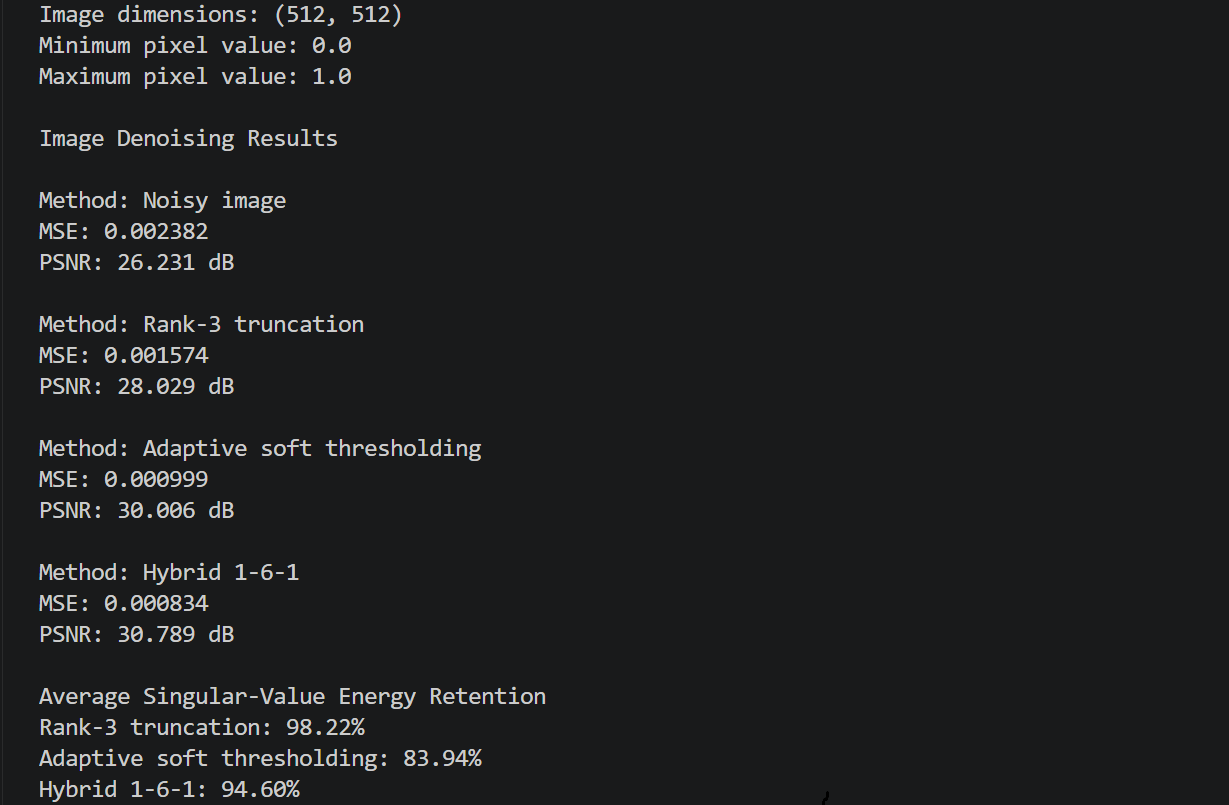
\includegraphics[width=0.6\textwidth]{console_output.png} 
    \caption{Console output of the program}
    \label{fig:console}
\end{figure}

\clearpage
\subsection*{Denoised Images}
The original image, the noisy image and the output of each method are shown in Figure~\ref{fig:rank3}, Figure~\ref{fig:adaptive} and Figure~\ref{fig:hybrid}.

\begin{figure}[h!]
    \centering
    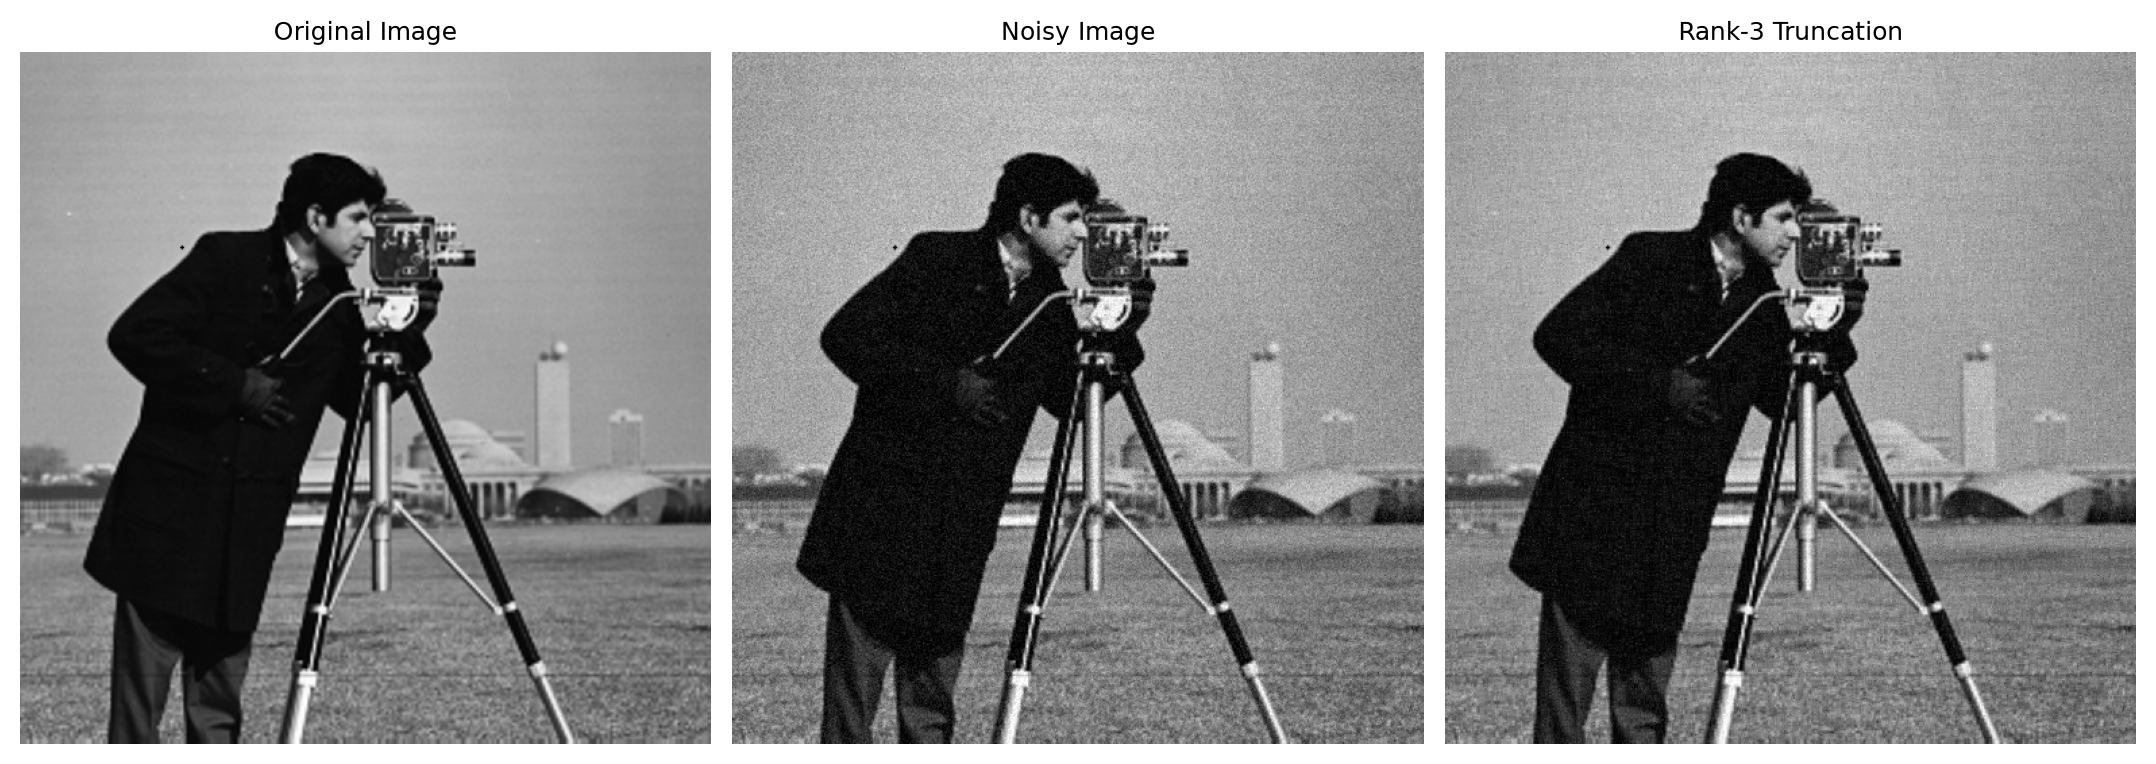
\includegraphics[width=0.9\textwidth]{fig_rank3.png} 
    \caption{Original image, noisy image and rank-3 truncation result}
    \label{fig:rank3}
\end{figure}
\begin{figure}[h!]
    \centering
    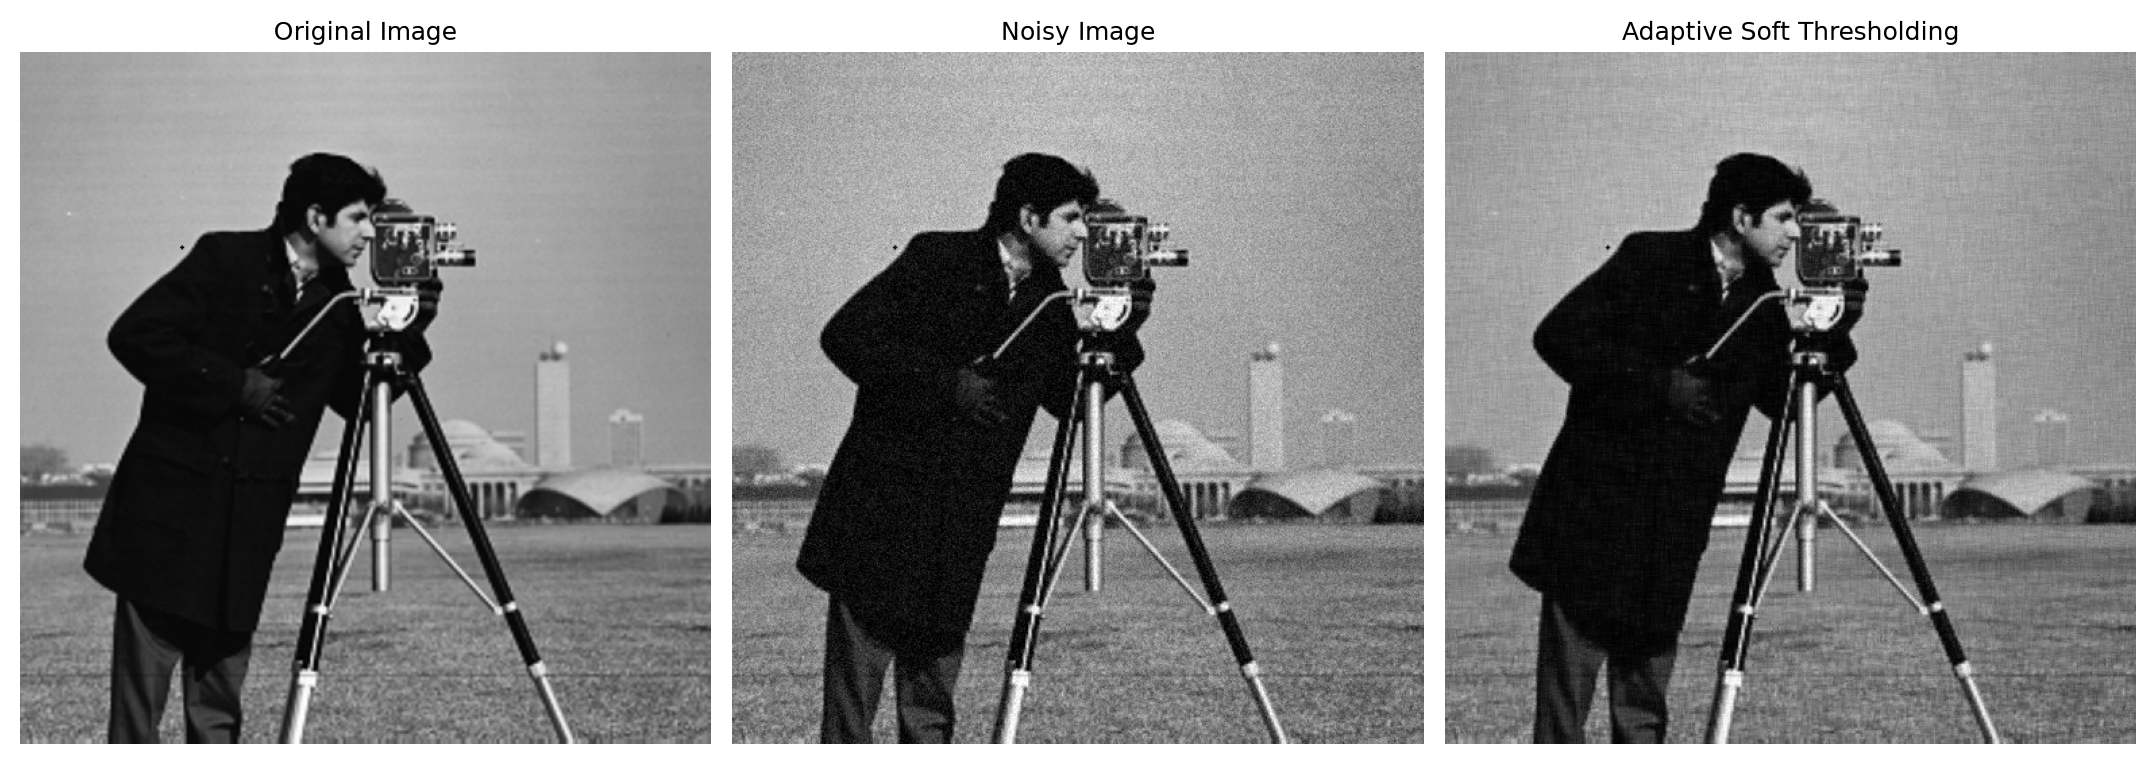
\includegraphics[width=0.9\textwidth]{fig_adaptive.png} 
    \caption{Original image, noisy image and adaptive soft thresholding result}
    \label{fig:adaptive}
\end{figure}
\begin{figure}[h!]
    \centering
    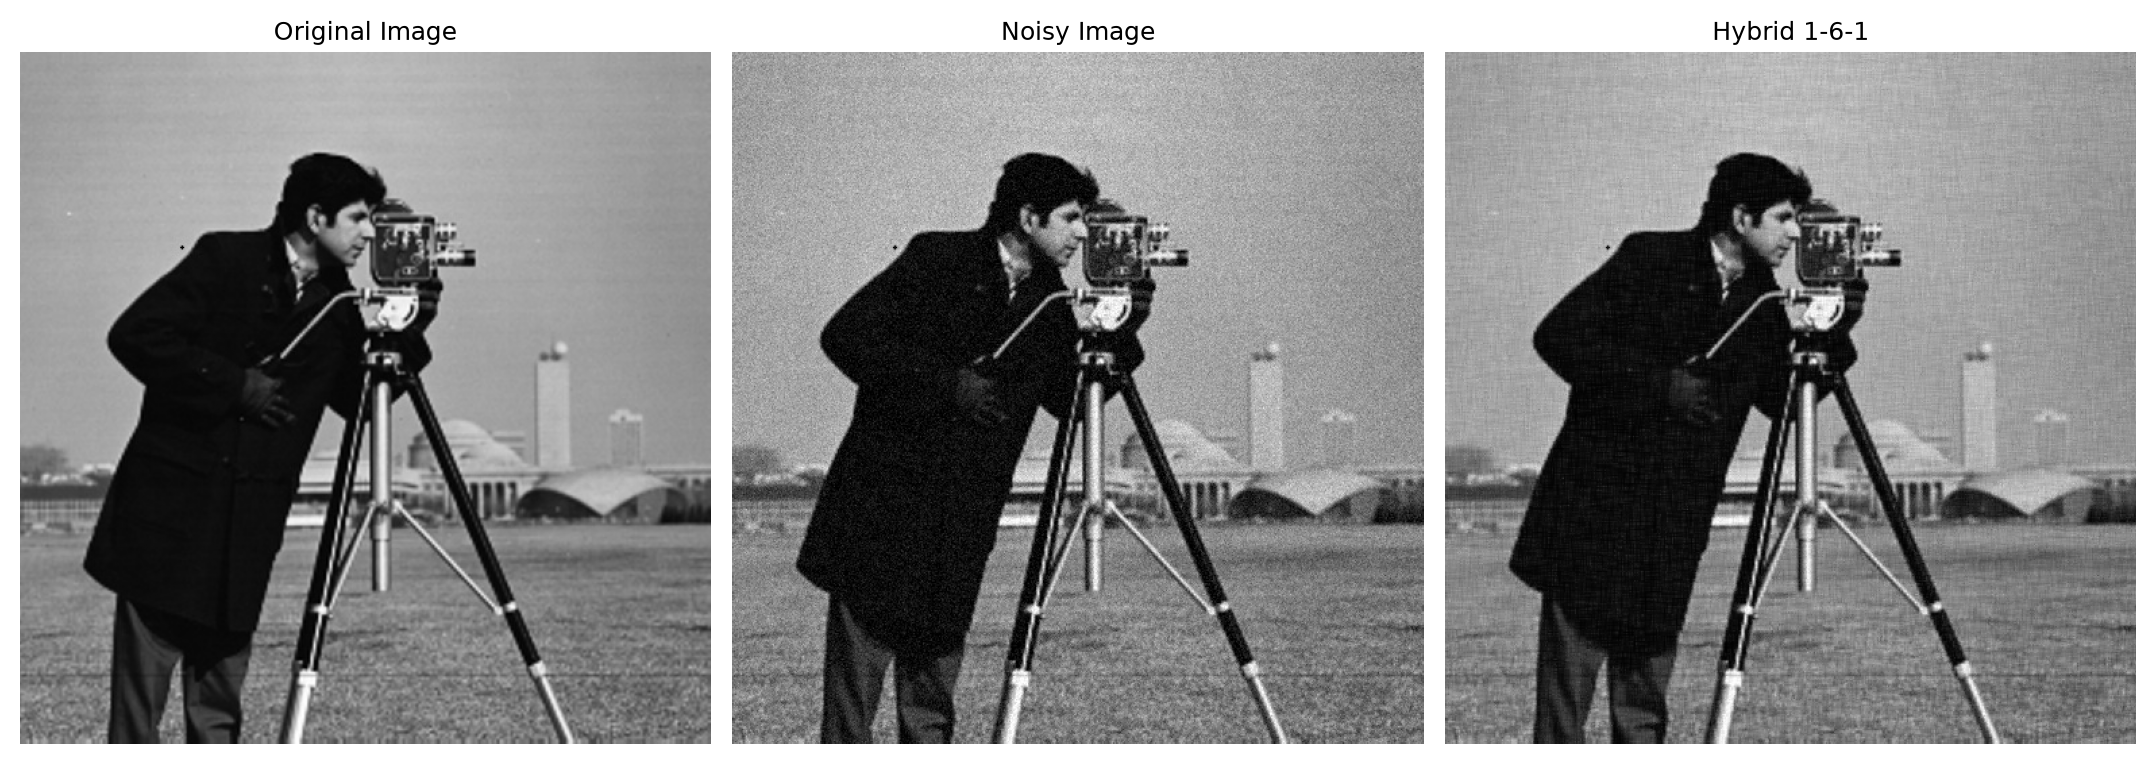
\includegraphics[width=0.9\textwidth]{fig_hybrid.png} 
    \caption{Original image, noisy image and hybrid 1-6-1 result}
    \label{fig:hybrid}
\end{figure}

\clearpage
\subsection*{Singular-Value Analysis}
The average singular values of the input patches and after each method are shown in Figure~\ref{fig:singular}, and the average energy retained is shown in Figure~\ref{fig:energy}.

\begin{figure}[h!]
    \centering
    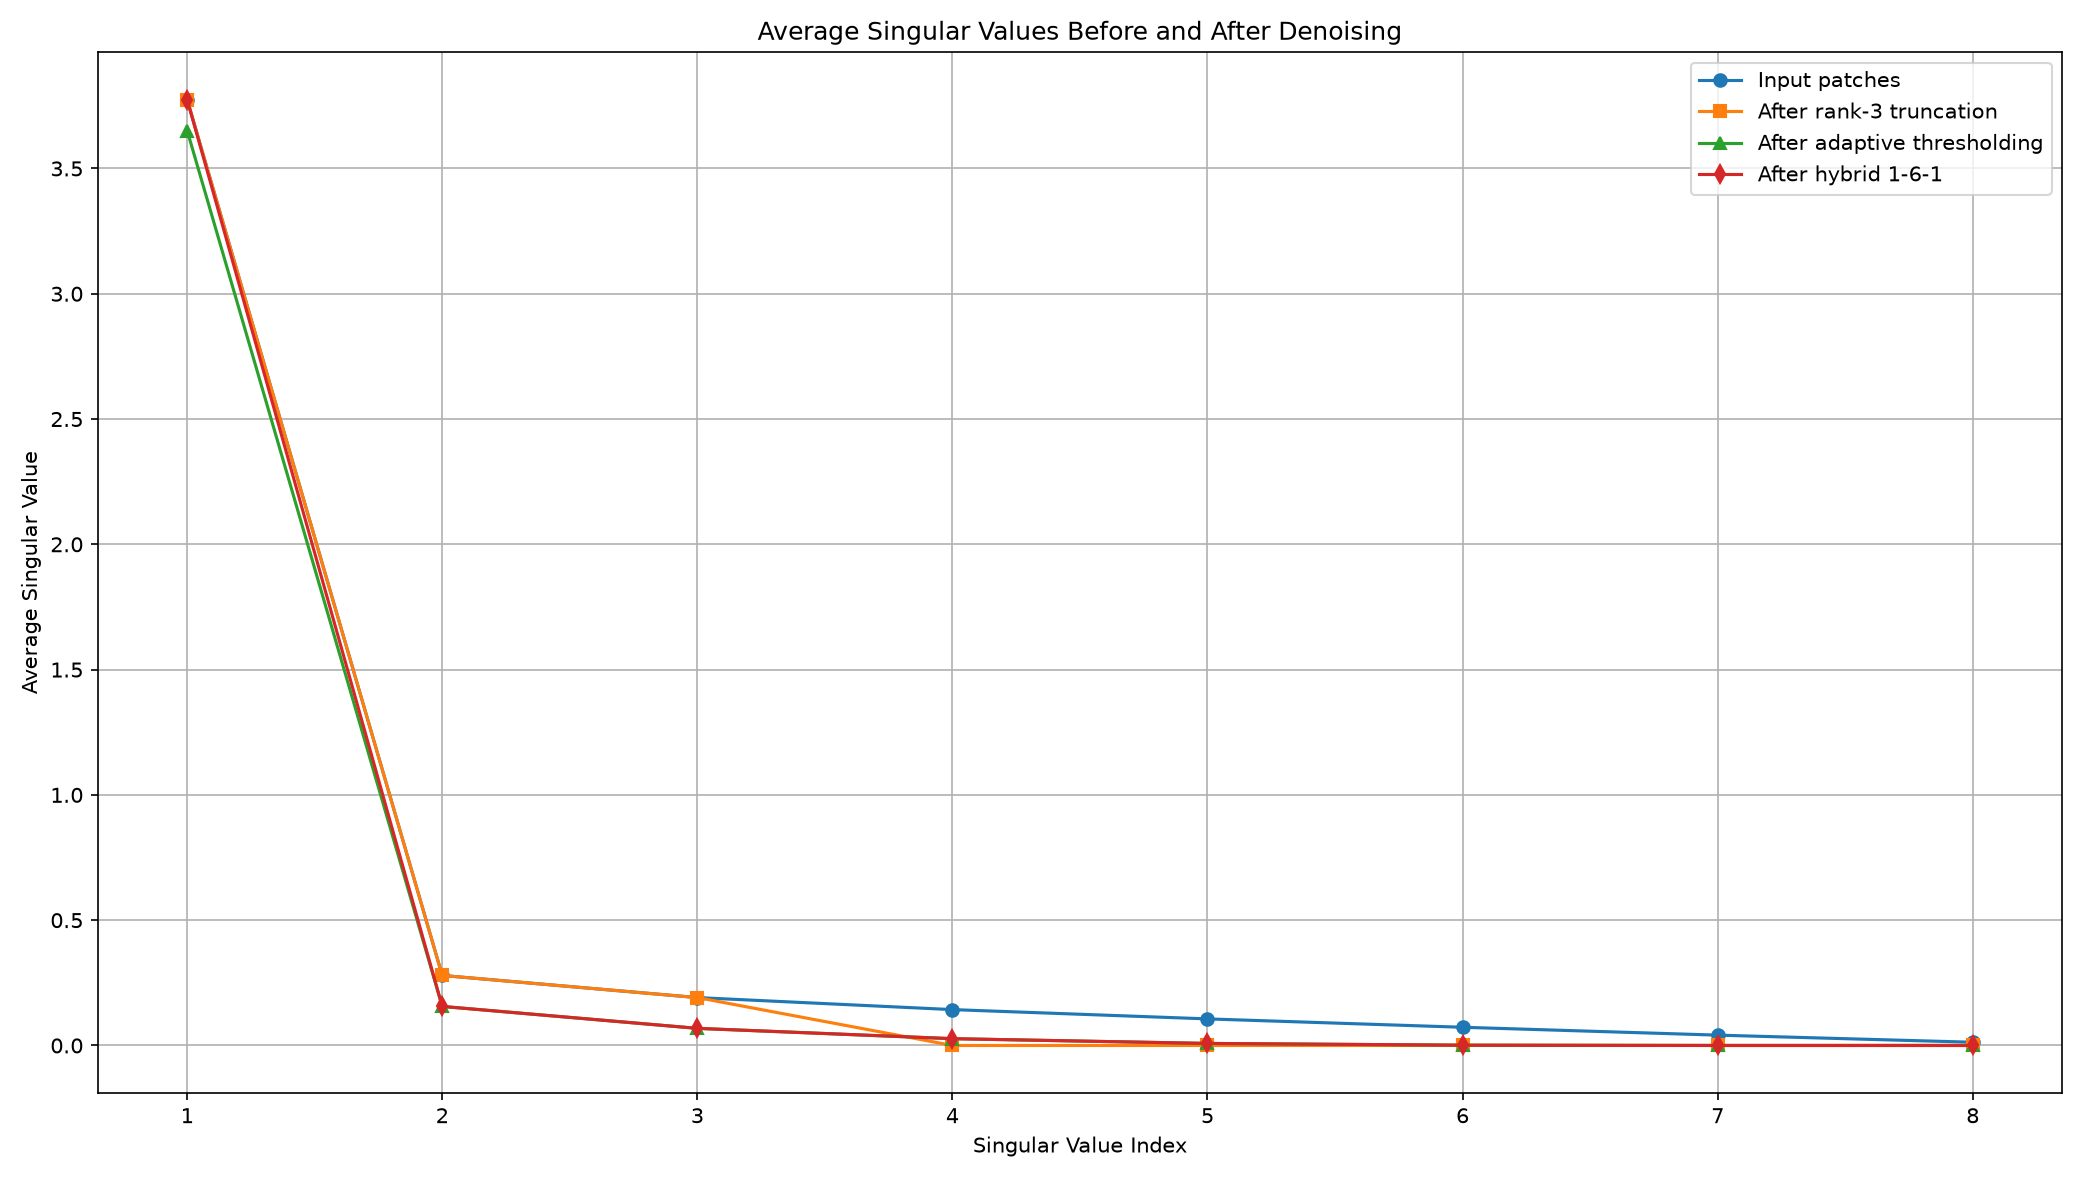
\includegraphics[width=0.85\textwidth]{fig_singular.png} 
    \caption{Average singular values before and after denoising}
    \label{fig:singular}
\end{figure}
\begin{figure}[h!]
    \centering
    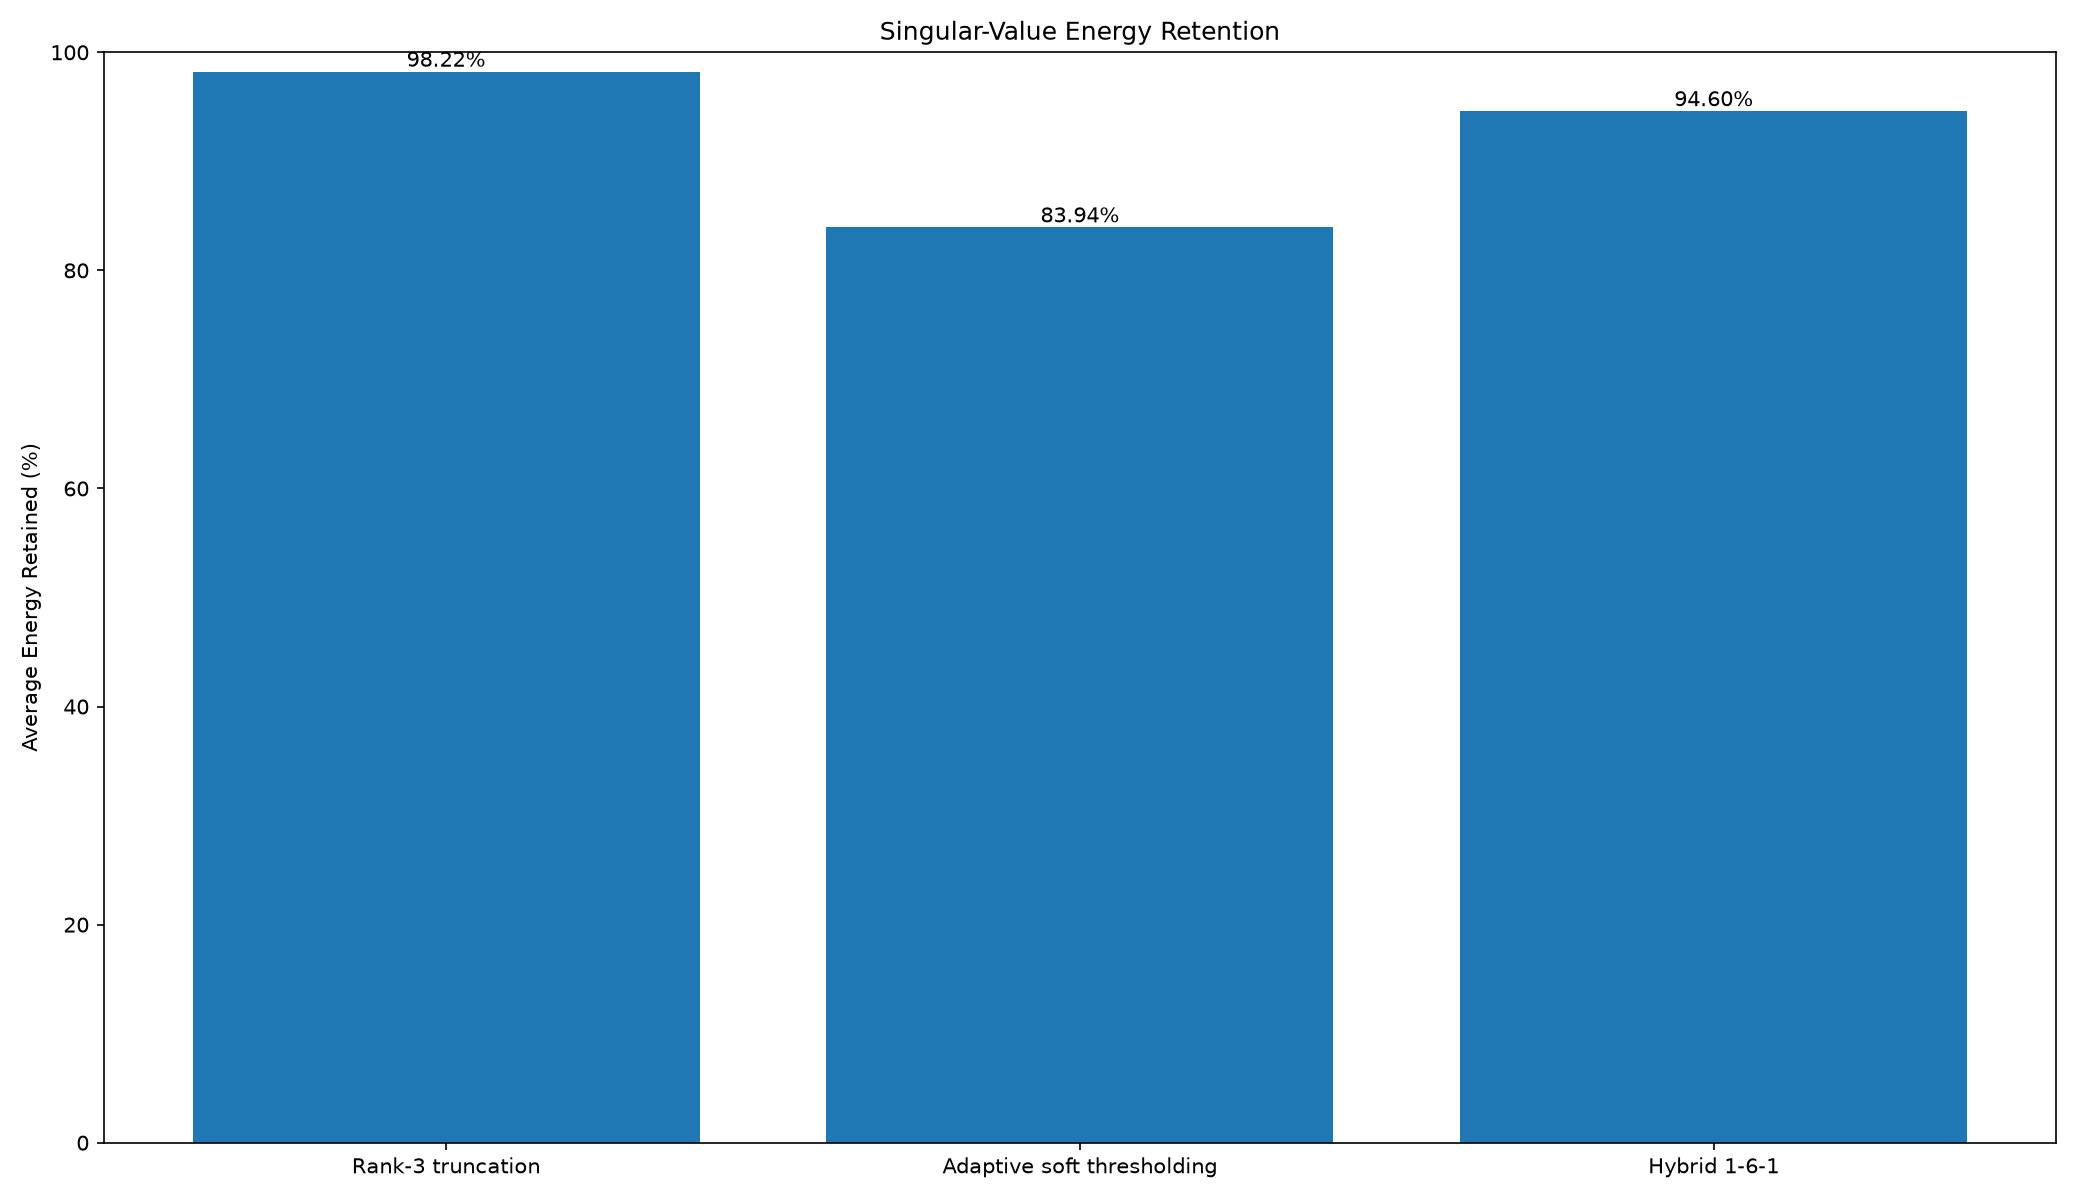
\includegraphics[width=0.85\textwidth]{fig_energy.png} 
    \caption{Singular-value energy retention}
    \label{fig:energy}
\end{figure}

\clearpage
\subsection*{Error Metrics}
The MSE and PSNR of the noisy image and of the three denoised images are compared in Figure~\ref{fig:mse} and Figure~\ref{fig:psnr}.

\begin{figure}[h!]
    \centering
    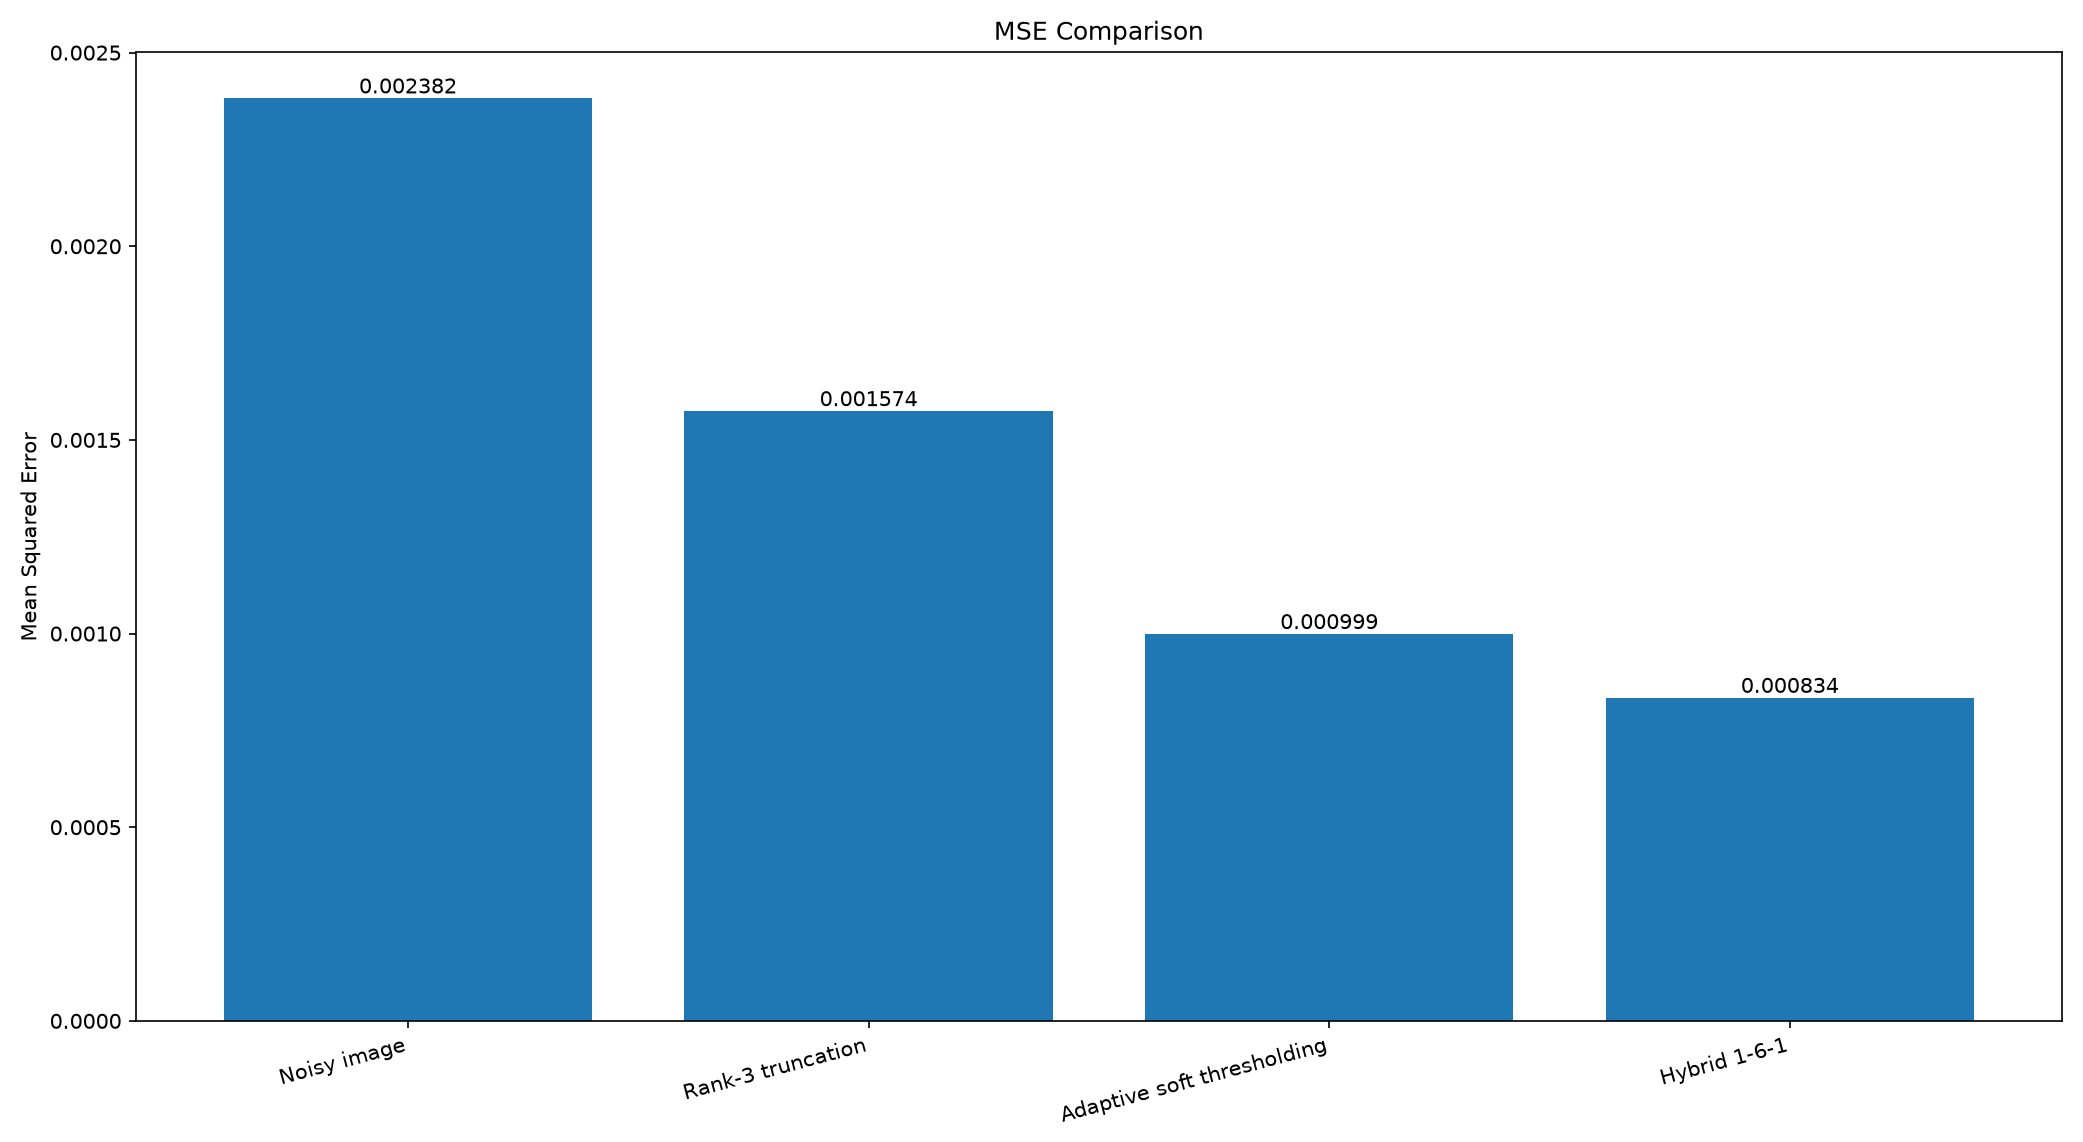
\includegraphics[width=0.85\textwidth]{fig_mse.png} 
    \caption{MSE comparison}
    \label{fig:mse}
\end{figure}
\begin{figure}[h!]
    \centering
    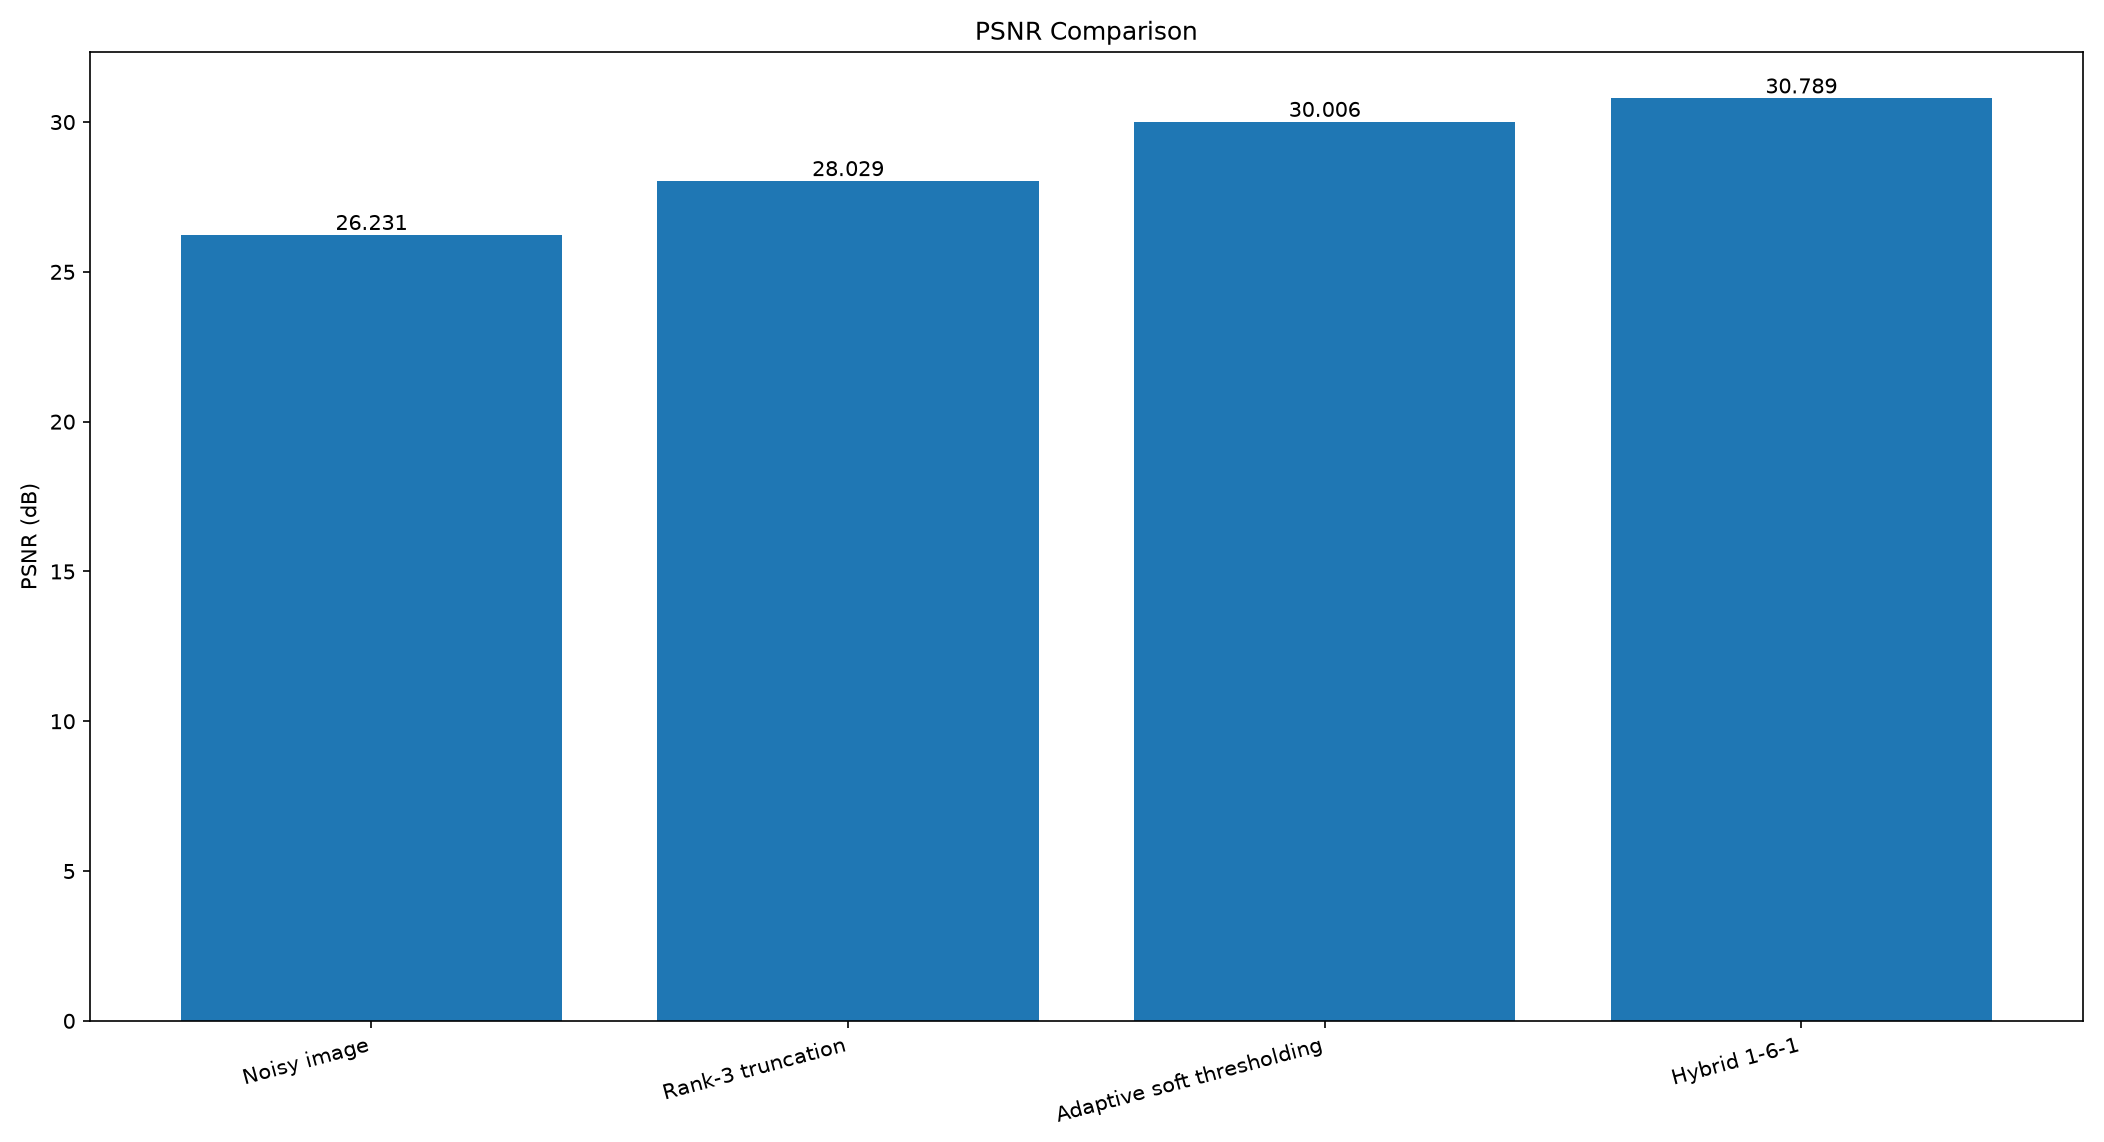
\includegraphics[width=0.85\textwidth]{fig_psnr.png} 
    \caption{PSNR comparison}
    \label{fig:psnr}
\end{figure}

\clearpage
\subsection*{Inference}
\begin{itemize}
    \item All three SVD-based methods improve on the noisy image. Relative to the noisy image's MSE, rank-3 truncation reduces the error by about 34\%, adaptive soft thresholding by about 58\% and the hybrid 1-6-1 method by about 65\%.
    \item Rank-3 truncation is the weakest of the three. It discards $s_4$ to $s_8$ but leaves $s_2$ and $s_3$ completely untouched, so the noise contained in those components is retained. This is why it keeps the most energy (98.22\%) yet gives the lowest PSNR of the three methods.
    \item Adaptive soft thresholding shrinks every singular value, including the dominant $s_1$ (visible as the slightly lower first point in Figure~\ref{fig:singular}). This removes noise from the small components but also reduces useful signal energy, leaving only 83.94\% energy retained.
    \item The hybrid 1-6-1 method gives the best PSNR (30.789 dB), about 0.78 dB higher than adaptive soft thresholding. It preserves the dominant first singular value exactly, shrinks the middle components, and removes the smallest one, so it protects the main structure of each patch while still suppressing noise.
    \item A higher energy retention does not mean better denoising: part of the retained energy in the small singular values is noise. The best method (hybrid) lies between the other two in energy retention.
\end{itemize}

\subsection*{Conclusion}
Patch-based SVD denoising is effective for removing Gaussian noise from images. Among the three methods tested, the hybrid 1-6-1 method gives the best result, raising the PSNR from 26.231 dB to 30.789 dB and lowering the MSE from 0.002382 to 0.000834. Combining an unmodified dominant singular value with adaptive soft thresholding of the smaller ones is therefore better than either hard rank truncation or uniform adaptive thresholding alone.

\end{flushleft}
\end{document}
